\documentclass[10pt, compress,usetitleprogressbar,aspectratio=1610, notes]{beamer}
% Si se quita "Notes" aparece sólo la presentación, sin notas.

\usepackage[spanish, es-tabla]{babel}
\usepackage{tikz}
\usepackage{listings}
\usepackage{showexpl}
\usepackage{booktabs}

% Solarized palette
\definecolor{solarizedBase03}{HTML}{002B36}
\definecolor{solarizedBase02}{HTML}{073642}
\definecolor{solarizedBase01}{HTML}{586e75}
\definecolor{solarizedBase00}{HTML}{657b83}
\definecolor{solarizedBase0}{HTML}{839496}
\definecolor{solarizedBase1}{HTML}{93a1a1}
\definecolor{solarizedBase2}{HTML}{EEE8D5}
\definecolor{solarizedBase3}{HTML}{FDF6E3}
\definecolor{solarizedYellow}{HTML}{B58900}
\definecolor{solarizedOrange}{HTML}{CB4B16}
\definecolor{solarizedRed}{HTML}{DC322F}
\definecolor{solarizedMagenta}{HTML}{D33682}
\definecolor{solarizedViolet}{HTML}{6C71C4}
\definecolor{solarizedBlue}{HTML}{268BD2}
\definecolor{solarizedCyan}{HTML}{2AA198}
\definecolor{solarizedGreen}{HTML}{859900}

\usetheme{epstfg}
\setbeamertemplate{note page}[compress]

\title{\LaTeX\ Crash Course}
\author{Guillermo Julián Moreno \and Pedro Valero Mejía}
\date{\today}

\lstset{
  backgroundcolor=\color{solarizedBase3},
  basicstyle=\ttfamily\footnotesize\color{solarizedBase01},
  breaklines=true,
  commentstyle=\color{solarizedBase0},
  stringstyle=\color{solarizedBase1},
  keywordstyle=\color{solarizedGreen},
  language={[LaTeX]TeX},
  morekeywords={textcolor,textsubscript,subsection,subsubsection,tableofcontents,includegraphics},
  columns = fullflexible,
  extendedchars = true,
  literate =
    {ñ}{{\~n}}1
    {í}{{\'i}}1
    {á}{{\'a}}1
    {é}{{\'e}}1
    {ó}{{\'o}}1
}
\def\inline{\lstinline[basicstyle=\ttfamily]}

\begin{document}

\maketitle
\note{Comentar un poco la estructura del taller.}

\section{¿Qué es \LaTeX?}
\note{Aunque probablemente muchos ya conozcáis \LaTeX, vamos a hacer una pequeña introducción a lo que es y cómo funciona. }

\begin{frame}
\frametitle{¿Qué es?}

Es un \textit{document typesetting system} o, en otras palabras, un sistema para escribir documentos (y en realidad más cosas, como esta presentación).

\begin{minipage}{0.5\textwidth}
Puntos fuertes:

\begin{enumerate}
\item No hay que preocuparse (demasiado) del formato.
\item Muy potente para escribir matemáticas.
\item Paquetes extra para hacer dibujos complejos, gráficas, algoritmos...
\item ¡Se puede programar!
\end{enumerate}
\end{minipage}
\begin{minipage}{0.4\textwidth}
\begin{flushright}
\begin{tikzpicture}[scale=0.9]
  \shade[top color=blue,bottom color=gray!50]
      (0,0) parabola (1.5,2.25) |- (0,0);
  \draw (2.3cm,0.8) node[align = left]
      {$\displaystyle\int\limits_0^{3/2} \!\!x^2\mathrm{d}x$};

  \draw[style=help lines] (0,0) grid (3.9,3.9)
       [step=0.25cm]      (1,2) grid +(1,1);

  \draw[->] (-0.2,0) -- (4,0) node[right] {$x$};
  \draw[->] (0,-0.2) -- (0,4) node[above] {$f(x)$};

  \foreach \x/\xtext in {1/1, 2/2, 3/3}
    \draw[shift={(\x,0)}] (0pt,2pt) -- (0pt,-2pt) node[below] {$\xtext$};

  \foreach \y/\ytext in {1/1, 2/2, 3/3}
    \draw[shift={(0,\y)}] (2pt,0pt) -- (-2pt,0pt) node[left] {$\ytext$};

  \draw (-.5,.25) parabola bend (0,0) (2,4) node[below right] {$x^2$};
\end{tikzpicture}
\end{flushright}
\end{minipage}

\note{
\begin{enumerate}
\item \LaTeX\ sabe perfectamente cómo colocar imágenes, alinear párrafos, poner títulos y más. Nosotros sólo decimos qué queremos hacer, y el sistema hace el resto. Incluso tenemos referencias automáticas, \LaTeX\ las formatea él sólo.
\item Otros editores de texto pueden poner ecuaciones matemáticas, pero las cosas se complican cuando queremos poner alguna alineada, o matrices, o... \LaTeX\ permite hacer todo eso y más.
\item Por ejemplo, la gráfica de la derecha está hecha con código \LaTeX, no hace falta cambiar de programa.
\item Se pueden desarrollar comandos propios, escribir nuestras propias ``plantillas'' de documento, y en definitiva hacer casi cualquier cosa.
\end{enumerate}

Aquí habría que comentar que esto lo hace muy buena elección para escribir documentos matemáticos, hacer prácticas (puedes tener plantillas ya hechas, y además no es difícil hacer un script que saque cosas en \LaTeX), o incluso tomar apuntes si (como nosotros) tienes los comandos para poder escribir rápido.
}

\end{frame}

\begin{frame}
\frametitle{¿Cómo funciona?}

\LaTeX\ no es un programa como Word, es más un lenguaje de programación. Nosotros escribimos un código, entremezclando comandos y texto, y luego lo compilamos para generar un PDF.

\begin{figure}[b]
\centering
\begin{minipage}{0.48\textwidth}
\centering
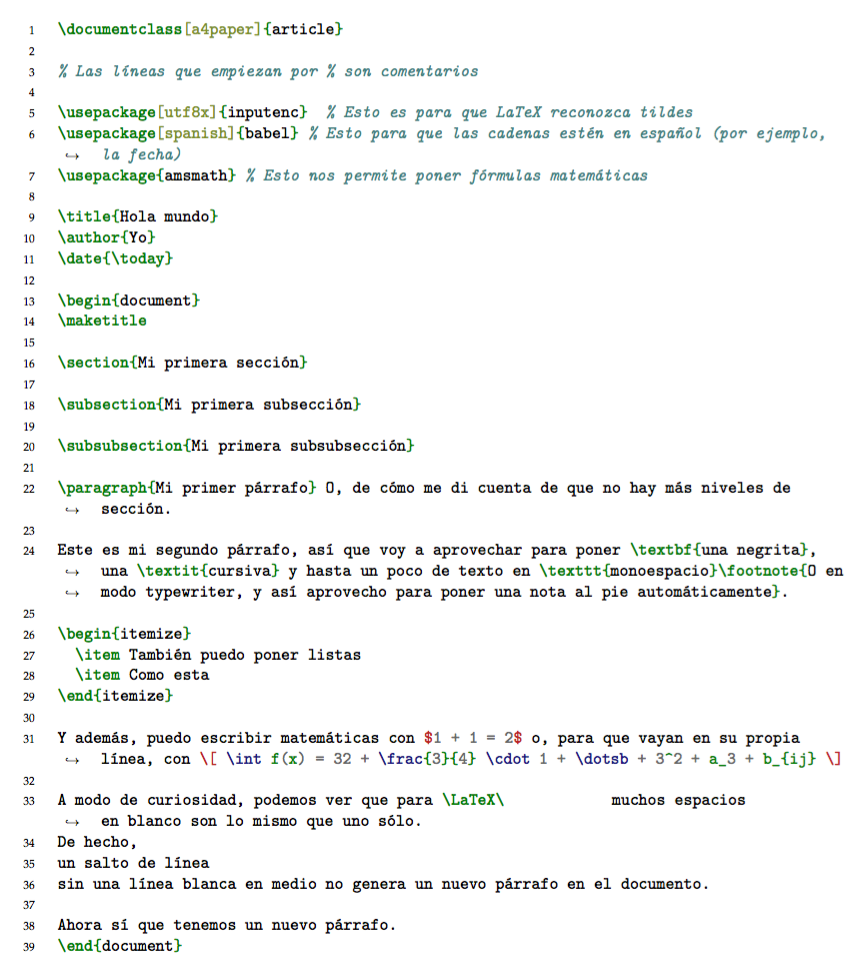
\includegraphics[height = 150pt]{CodigoLatex.png}
\end{minipage}
\begin{minipage}{0.48\textwidth}
\centering
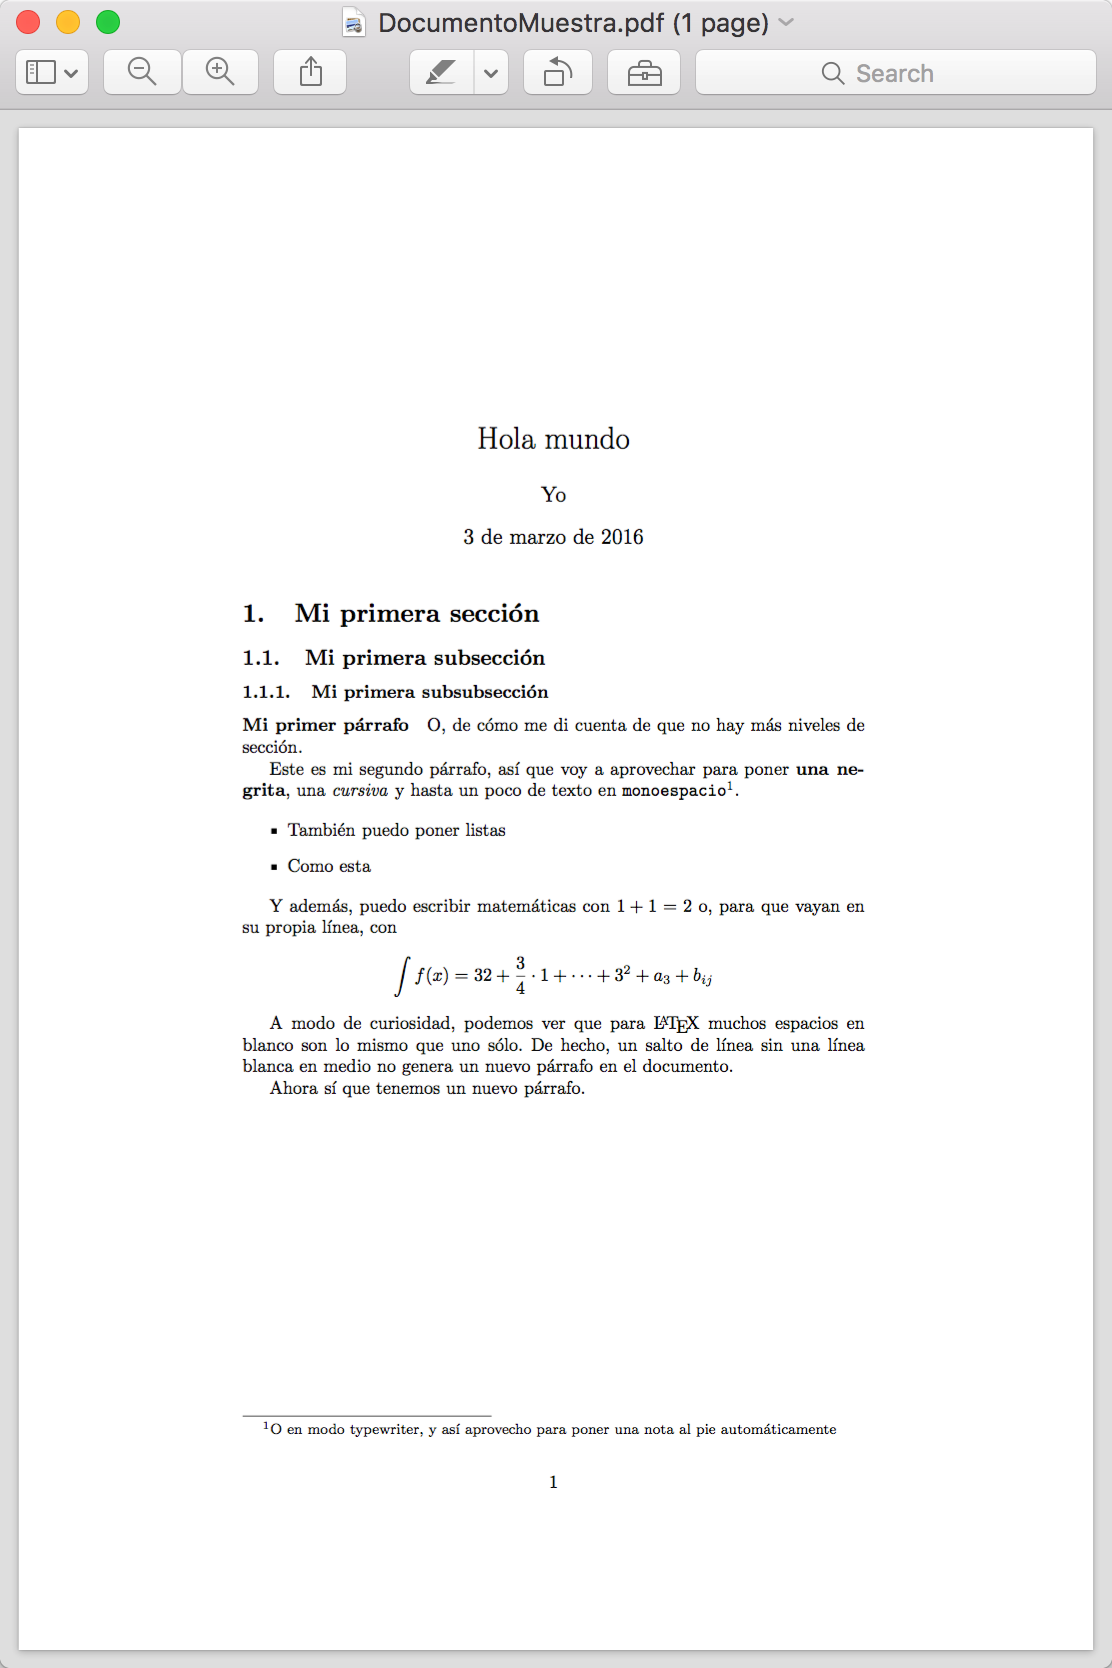
\includegraphics[height = 150pt]{DocumentoFinal.png}
\end{minipage}
\end{figure}

\note{Comentar las ``desventajas'' de usar un compilador: fallos de compilación, tener que hacer varias pasadas para tener todo bien (índice, referencias)... También habría que mencionar \textit{latexmk}, que hace todo esto él solito.

Por supuesto, el compilador tiene ventajas, y la principal es la automatización y la rapidez. Podemos usar el editor que queramos, no hay problemas de compatibilidad...
}
\end{frame}

\begin{frame}
\frametitle{¿Qué necesito para usarlo?}

\begin{itemize}
\item Un compilador y una distribución \LaTeX.
\begin{itemize}
\item Linux: \textit{texlive}.
\item Windows: \textit{MikTeX}.
\item OS X: \textit{MacTeX}.
\end{itemize}
\item Un editor. Para principiantes, \textbf{TeXStudio} viene muy bien: tiene asistentes, autocompletado y muchas ayudas. También se puede usar otros editores, como Sublime Text, Vim o Emacs.
\item Ganas, Google y TeX.StackExchange.
\end{itemize}

\note{\begin{itemize}
\item Basta con buscar ``Latex SO'' en Google para encontrar fácilmente cómo instalarlo. Mencionar que en OS X también se puede usar \textit{texlive} a través de MacPorts / Homebrew.
\item TeXStudio viene muy, muy bien. Sublime también está genial, sobre todo con plugins LaTeXing o LaTeXTools.
\item Como siempre, aunque en este caso el nivel de TeX.StackExchange es incluso mejor del de StackOverflow. Cualquier problema que tengáis ya lo habrá sufrido alguien y ya estará resuelto por ahí.
\end{itemize}}
\end{frame}

\section{Sintaxis y comandos}

\note{Vamos a hacer una introducción rápida a la sintaxis de \LaTeX y a los comandos que tiene. Como os comentamos al principio, luego os vamos a pasar algunos ejemplos con cosas que se pueden hacer con \LaTeX\ para que probéis y veáis cómo funciona.}

\begin{frame}[fragile]
\frametitle{Documentos \LaTeX}
\begin{minipage}{0.45\textwidth}
Un documento \LaTeX\ no es más que un archivo de texto plano, habitualmente con la extensión \textit{.tex}, que se compila después a PDF.
\vspace{15pt}

Estructura:
\begin{enumerate}
\item Preámbulo: qué tipo de documento queremos hacer, qué paquetes cargamos, tipo de letra, márgenes, etc.
\item Contenido: el texto que saldrá después en el PDF.
\end{enumerate}
\end{minipage}
\hspace{15pt}
\begin{minipage}{0.45\textwidth}
\begin{lstlisting}
\documentclass[a4paper,11pt]{article}

\usepackage[spanish]{babel}
\usepackage[T1]{fontenc}
\usepackage[utf8x]{inputenc}


\begin{document}
\section{Hello World!}

Hola, \textbf{mundo}.

\end{document}
\end{lstlisting}
\end{minipage}

\note{Los comandos en \LaTeX\ empiezan por \textbackslash. Los comandos del principio dicen a \LaTeX\ qué tipo de documento queremos (\textit{article} en este caso, pero también puede haber \textit{book, report} entre otros), y qué \textit{plugins} usar.

Hay algunos comandos especiales, llamados entornos, que empiezan con begin/end entorno, como el \textit{document}, y sirven para marcar ``regiones''. Por ejemplo, podemos tener begin/end theorem, o figure, etc.}

\end{frame}

\begin{frame}[fragile]
\frametitle{Formato de texto}

\begin{tabular}{r|l}
Formato & Código \\ \toprule
\textbf{Negrita} & \inline!\textbf{Negrita}! \\
\textit{Cursiva} & \inline!\textit{Cursiva}! \\
\texttt{Monospace} & \inline!\texttt{Monospace}! \\
Letra {\large grande} o {\small pequeña} & \inline!Letra {\large grande} o {\small pequeña}! \\
\textcolor{red}{Rojo} & \inline!\textcolor{red}{Rojo}! \\
\textsuperscript{Super}\textsubscript{Sub}índice & \inline!\textsuperscript{Super}\textsubscript{Sub}índice!
\end{tabular}

\note{}
\end{frame}

\begin{frame}[fragile]
\frametitle{Estructura: secciones, subsecciones, \ldots}

Para añadir nuevas secciones, subsecciones o subsubsecciones al documento sólo hay que añadir los comandos correspondientes: \inline!\section{Título}, \subsection{Título}! y \inline!\subsubsection{Título}!.

\LaTeX\ se encarga del resto: la numeración y tabla de contenidos (que se imprime con el comando \inline!\tableofcontents!) salen automáticamente.

\note{Es una gran ventaja el no tener que preocuparnos de nada. Podemos añadir nuevas secciones, cambiarlas de sitio o de título y no pasará nada: \LaTeX\ arreglará la numeración las referencias para que todo siga siendo coherente.}
\end{frame}

\begin{frame}[fragile]
\frametitle{Estructura: Párrafos}

\begin{minipage}{0.45\textwidth}
En \LaTeX, los párrafos se crean sólo
con líneas en blanco.
Una nueva línea
no cambia de párrafo.
\vspace{10pt} % Trampa, por no cambiar el espacio entre párrafos en todo el documento.

Pero si dejamos una en blanco sí hay cambio.
\end{minipage}
\hspace{10pt}
\begin{minipage}{0.45\textwidth}
\begin{lstlisting}
En \LaTeX, los párrafos se crean sólo
con líneas en blanco.
Una nueva línea
no cambia de párrafo.

Pero si dejamos una en blanco sí hay cambio.
\end{lstlisting}
\end{minipage}
\vspace{10pt}

Aunque se puede cambiar de línea con \inline!\\!, no es recomendable: no hace el sangrado y no pone la separación entre párrafos correspondiente.

\note{\LaTeX\ sabe bastante mejor que nosotros dónde cortar líneas y cómo organizar los párrafos para que todo quede bien. Por eso es importante separar con líneas en blanco para marcar los nuevos párrafos.

Entre los ejercicios hay alguno para personalizar cómo quedan los párrafos y la separación.}
\end{frame}

\begin{frame}[fragile]
\frametitle{Listas}
\begin{minipage}{0.45\textwidth}
\begin{enumerate}
\item Listas numeradas
\item Igual que antes, la numeración es automática.
\end{enumerate}

\begin{itemize}
\item Por supuesto, también puede haber listas sin numerar.
\end{itemize}
\end{minipage}
\hspace{10pt}
\begin{minipage}{0.45\textwidth}
\begin{lstlisting}
\begin{enumerate}
\item Listas numeradas
\item Igual que antes, la numeración es automática.
\end{enumerate}

\begin{itemize}
\item Por supuesto, también puede haber listas sin numerar.
\end{itemize}
\end{lstlisting}
\end{minipage}
\end{frame}

\begin{frame}[fragile]
\frametitle{Imágenes}

\LaTeX\ se encarga de poner las imágenes donde mejor venga. La sintaxis es la siguiente:

\begin{lstlisting}
\begin{figure}[hbtp]  % Dónde colocar la imagen
\centering            % Todo centrado
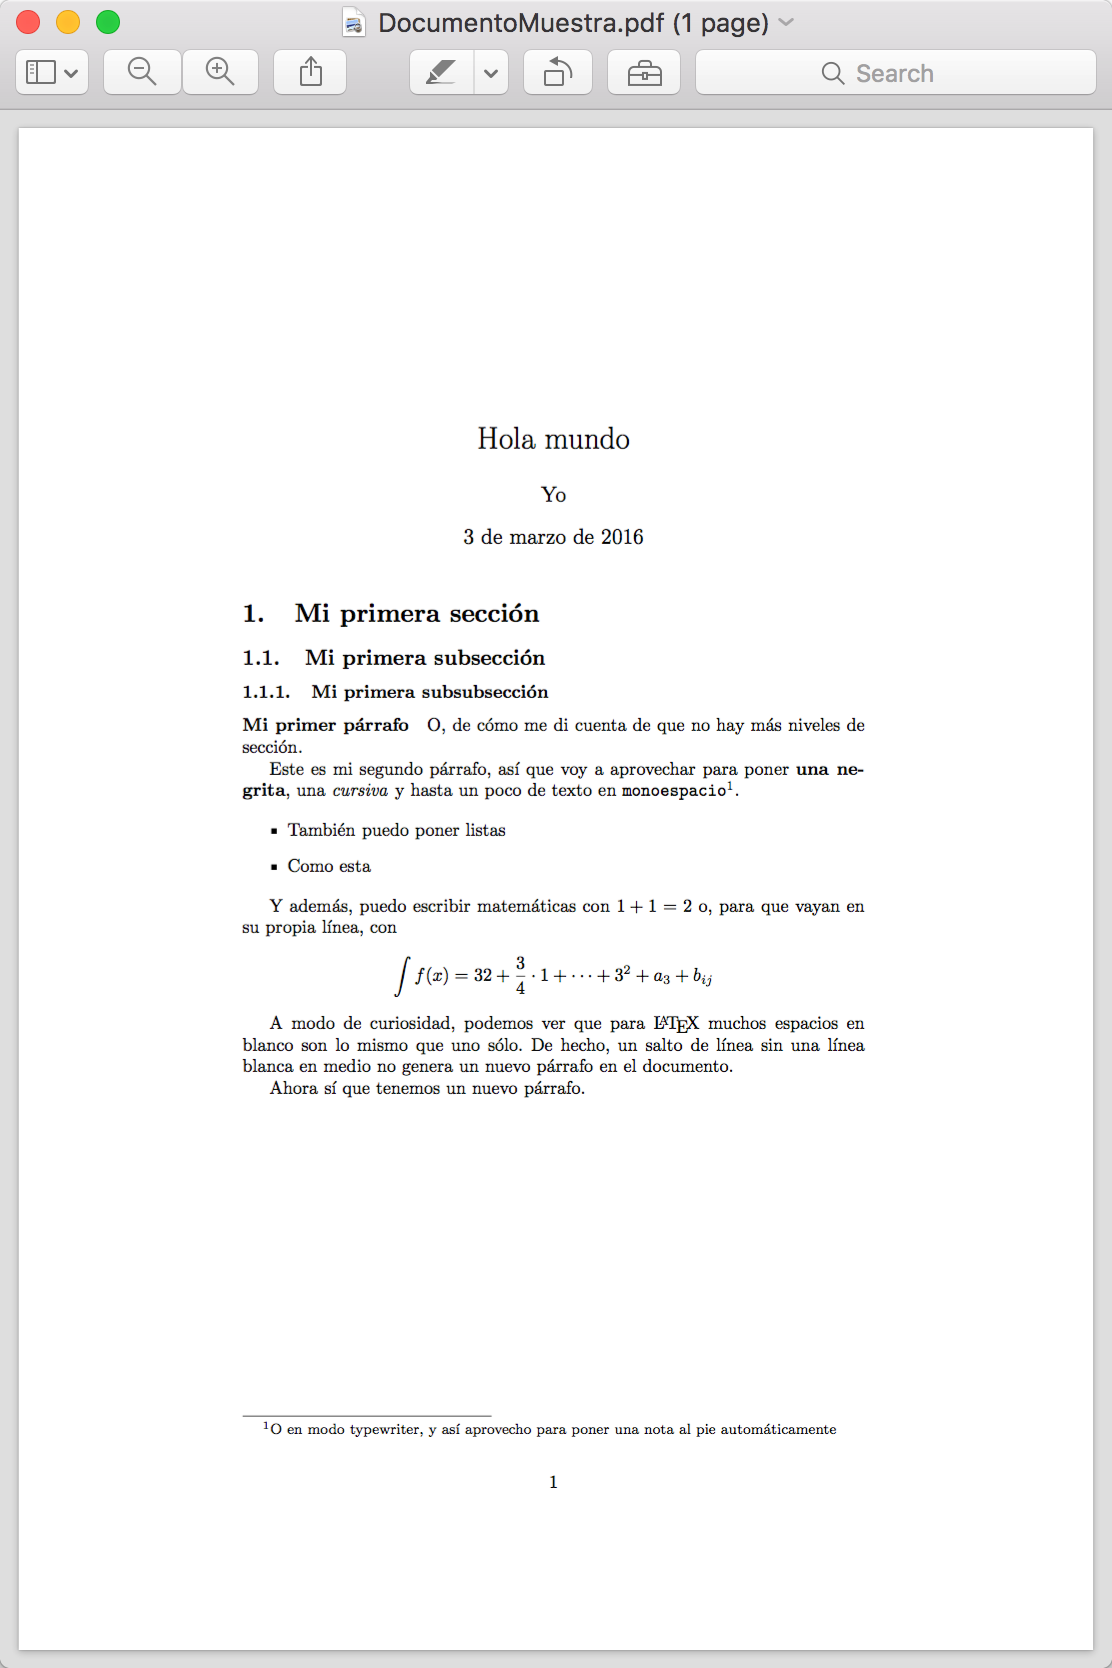
\includegraphics[width = 0.8\textwidth]{DocumentoFinal.png}
\caption{Leyenda}     % Leyenda para la imagen
\label{fig:Documento} % Para referencias posteriores
\end{figure}
\end{lstlisting}

El \inline!hbtp! indica a \LaTeX\ dónde quieres colocar la imagen, en orden de prioridad: \textit{\textbf{h}ere}, \textit{\textbf{t}op}, \textit{\textbf{b}ottom}, \textit{\textbf{p}age} (en una página separada).

\note{
  La ventaja de usar el entorno \textit{figure} es que no hay que preocuparse, como en Word, que al añadir una nueva línea en el documento se destroce todo varias páginas más abajo.

  El problema es que no siempre se pone la imagen donde queremos. A veces se puede jugar con eso moviéndola un párrafo para arriba o para abajo en el código. De todas formas, en general es mejor dejar a \LaTeX\ ponerlas donde quiera y usar las referencias y etiquetas.
}

\end{frame}

\begin{frame}[fragile]
\frametitle{Tablas}

Al igual que las imágenes, las tablas se ponen en entornos flotantes que \LaTeX\ decide después dónde colocar.

\begin{minipage}{0.45\textwidth}
\begin{table}[hbtp]
\centering
\begin{tabular}{r | c || l }
Celda 1 & Celda 2 & Celda 3 \\ \hline
1 & 2 & 3
\end{tabular}
\caption{Leyenda}
\label{tbl:TablaEjemplo}
\end{table}
\end{minipage}
\hspace{10pt}
\begin{minipage}{0.45\textwidth}
\begin{lstlisting}
\begin{table}[hbtp]
\centering
\begin{tabular}{r | c || l }
Celda 1 & Celda 2 & Celda 3 \\ \hline
1 & 2 & 3
\end{tabular}
\caption{Leyenda}
\label{tbl:TablaEjemplo}
\end{table}
\end{lstlisting}
\end{minipage}

\note{La principal diferencia con el entorno \textit{figure} es que en lugar de meter la imagen, escribimos la tabla a mano. Es un poco más engorroso que con Excel, por ejemplo.

El primer argumento de \textit{tabular} es la especificación de columnas: r,c,l indican la alineación del texto en las celdas, y las barras indican los bordes.

Cada celda se separa con un ampersand, y las filas se separan con las dos barras. Además, se pueden poner líneas horizontales con hline.}

\end{frame}

\begin{frame}[fragile]
\frametitle{Etiquetas y referencias}

\begin{minipage}{0.45\textwidth}
Las etiquetas se definen con
\label{etiqueta}. Después,
se pueden referenciar, como
antes la tabla \ref{tbl:TablaEjemplo},
o la que acabamos de definir en la
página \pageref{etiqueta}.
\end{minipage}
\hspace{10pt}
\begin{minipage}{0.45\textwidth}
\begin{lstlisting}
Las etiquetas se definen con
\label{etiqueta}. Después,
se pueden referenciar, como
antes la tabla \ref{tbl:TablaEjemplo},
o la que acabamos de definir en la
página \pageref{etiqueta}.
\end{lstlisting}
\end{minipage}

Pequeño inconveniente: a veces hay que compilar varias veces para que las referencias salgan bien.

\note{Como el compilador de \LaTeX\ es de una única pasada, lo que hace es escribir las etiquetas que se va encontrando en un archivo auxiliar, de donde las recupera cuando tiene que poner una referencia. Si la referencia está antes que la etiqueta, hay que hacer dos pasadas: una para que sepa dónde está la etiqueta y escriba en el archivo, y otra para que lea ese archivo auxiliar y pueda poner la referencia correcta.}

\end{frame}

\section{Matemáticas}

\end{document}
